\section{Dialog \& Schema Representation and Inference~(Q1)}
\label{sec:sgd:models}
In this section, we focus on the model architecture for matching
dialog history with schema descriptions using pretrained
BERT~\cite{devlin2019bert}~\footnote{We use BERT-base-cased for all
  main experiments. Other pretrained language models can be easily adapted to our study}. To support four subtasks,
we first extend \DE and \CE~to support both sentence-level matching and token-level
prediction. Then we propose an additional \FE strategy to get faster
inference without sacrificing much accuracy. We summarize different
architectures in~\autoref{fig:encoders}. Then we show the
classification head and results for each subtask.

\begin{figure}[!t]
\centering
  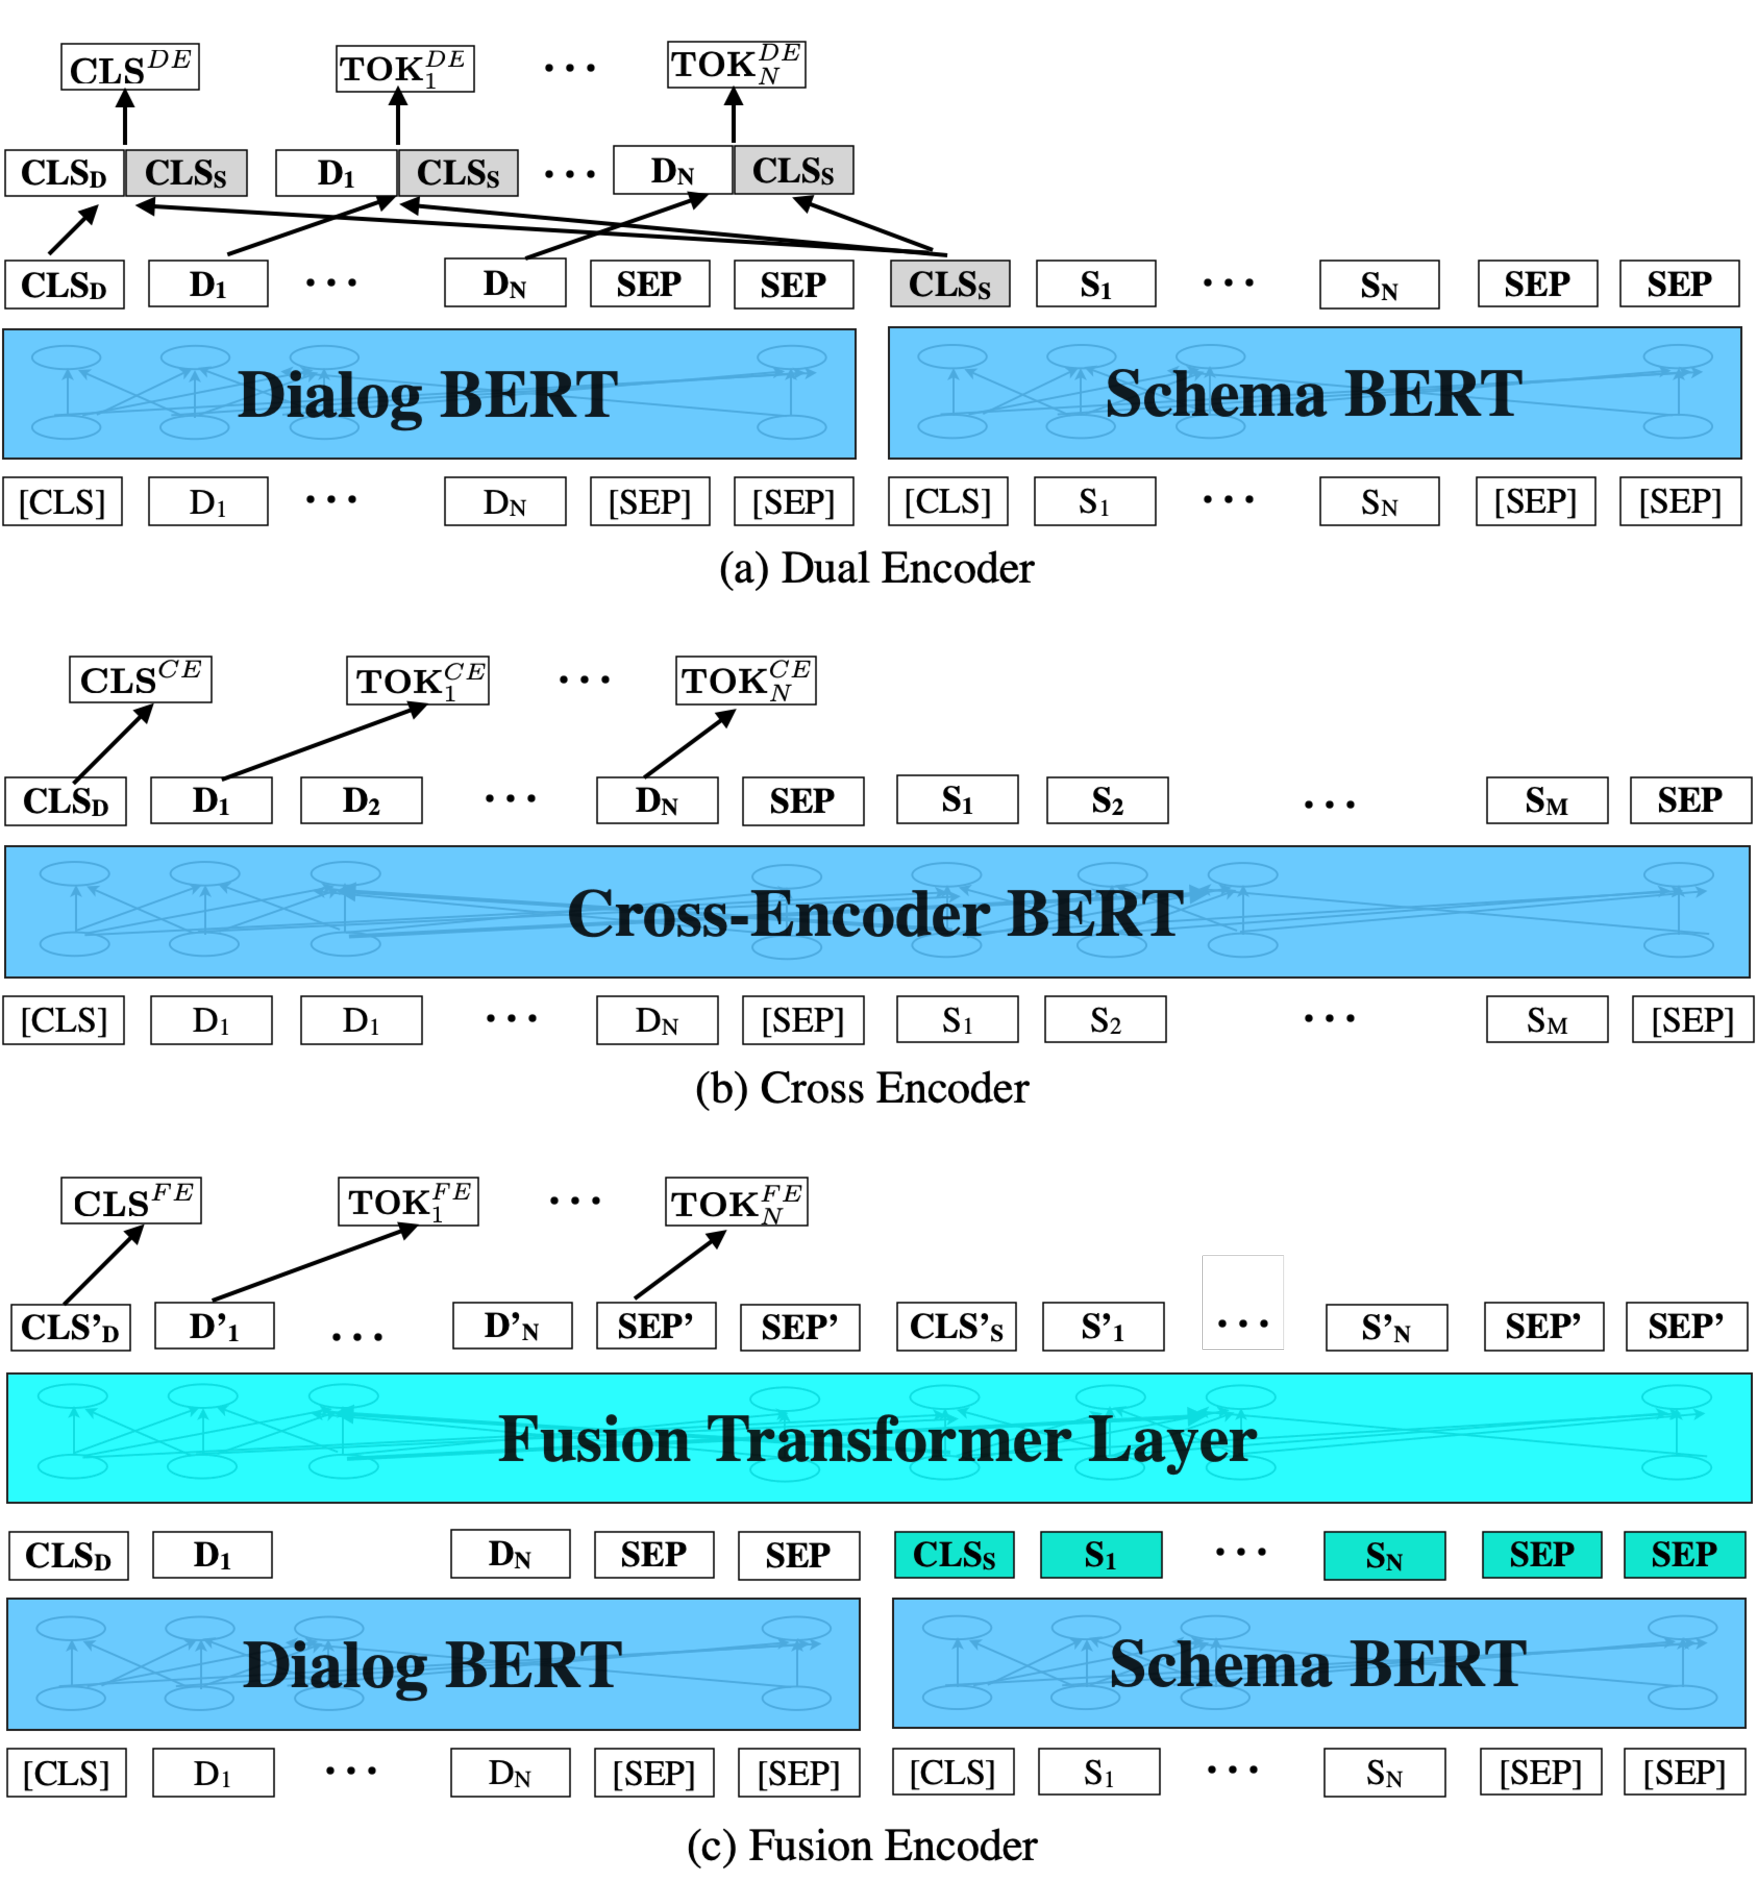
\includegraphics[width=0.90\textwidth]{all-encoders.pdf}
  \caption{\label{fig:encoders} Dual-Encoder, Cross-Encoder and Fusion Encoder, shaded block will be cached during training}
\end{figure}

\subsection{Encoder Architectures}
\label{ssec:encoder-arch}
\Paragraph{Dual-Encoder} It consists of two separate BERTs to encode
dialog history and schema description respectively, as
Figure~\ref{fig:encoders}~(a). We follow the setting in the official
baseline provided by DSTC8 Track4~\cite{rastogi2020schema}. We first
use a fixed BERT to encode the schema description once and cached the
encoded schema $\CLS_{S}$. Then for sentence-level representation, we
concatenate dialog history representation $\CLS_{D}$ and candidate
schema representation $\CLS_{S}$ as the whole sentence-level
representation for the pair, denoted as~${\CLS^{DE}}$.  For
token-level representation, we concatenate the candidate schema
$\CLS_{S}$ with each token embedding in the dialog history, denoted
as~${\TOK^{DE}}$.\footnote{A schema-aware dialog token embedding can
  also be computed by attention or other method for span-based
  detection tasks~\cite{humeau2019poly, noroozi2020fast}} Because
the candidate schema embeddings are encoded independently from the
dialog context, they can be pre-computed once and cached for fast
inference.

\Paragraph{Cross-Encoder} Another popular architecture as
Figure~\ref{fig:encoders}~(b) is \CE, which concatenates the dialog
and schema as a single input, and encodes jointly with a single
self-attentive encoder spanning over the two segments.  When using
BERT to encode the concatenated sentence pair, it performs
full~(cross) self-attention in every transformer layers, thus offer
rich interaction between the dialog and schema. BERT naturally
produces a summarized representation with [CLS]
embedding~${\CLS^{CE}}$ and each schema-attended dialog token
embeddings~${\TOK^{CE}}$. Since the dialog and schema encoding always
depend on each other, it requires recomputing dialog and schema
encoding for multiple times, thus much slower in inference.
%
%\subsubsection{Poly-Encoder}
%\label{sssec:poly-encoder}
%Poly-Encoder~\citet{humeau2019poly} was proposed to response selection
%and article retrieval tasks, where a pair of context and candidate
%sentences need to be encoded. Extending to our schema-guided dialog
%task, the pair of text are dialog context and schema
%descriptions. Poly-Encoder seperately encode the schemas, thus can
%precompute and cache all the schema embedding, which is adopted from
%the Dual-Encoder, thus efficient for training and inference; Then for
%context dialog encoding, Poly-Encoder borrow the cross attention
%ability from Cross-Encoder, it first predicts $m$ different
%representation vector for dialog context rather than a single vector
%in Dual-Encoder, then it attend over them using the precomputed single
%schema as a query, finally sum up all the weighted dialog context as
%schema-aware dialog representation.

\Paragraph{Fusion-Encoder} In Figure~\ref{fig:encoders}~(c), similar
to \DE, \FE also encodes the schema independently with a fixed BERT
and finetuning another BERT for dialog encoding. However, instead of
caching a single [CLS] vector for schema representation, it caches {\bf all
token representation} for the schema including the [CLS] token. What's
more, to integrate the sequences dialog token representation with
schema token representation, an extra stack of transformer layers are
added on top to allow token-level fusion via self-attention, similar
to \CE. The top transformer layers will produce embeddings for each
token~${\TOK^{FE}}$ including a schema-attended
~${\CLS^{FE}}$ of the input [CLS] from the dialog
history. With cached schema token-level representations, it can
efficiently produce schema-aware sentence- and token-level
representation for each dialog-schema pairs.

\subsection{Models for Factorized Subtasks}
\label{ssec:models-overview}
All the above 3 encoders will produce both sentence- and token-level
representations for a given sentence pair. In this section,
we abstract them as two representations~\CLS~and~\TOK, and present the
universal classification heads to make decisions for each subtask.
%Especially, slots from previous dialog state can be carried over to
%the next dialog state, cross the same or different dialog state. For
%example, the hotel name in the hotel-booking service can be carried
%over to the detination in the taxi-service, while the amount in
%``MakePayment" cannot be carried to ``RequestPayment". The strategies
%for those common dialog state tracking strategies such as two-stage,
%overwriting memory, end2end has been widely studied in previous work.

\Paragraph{Active Intent} To decide the intent for current dialog
turn, we match current dialog history $D$ with each intent
descriptions $I_{0}...I_{k}$. For each dialog-intent pair $(D,I_{k})$,
we project the final sentence-level \CLS~representation to a single
number $P_{I_{k}}^{active}$ with a linear layer follows a sigmoid
function. We predict \textit{"NONE"} if the $P_{I_{k}}^{active}$ of
all intents are less than a threshold 0.5, which means no intent is
active. Otherwise, we predict the intent with largest
$P_{I_{k}}^{active}$. We predict the intent for each turn
independently without considering the prediction on previous turns.

\Paragraph{Requested Slot} As in Figure~\ref{fig:schema-dst},
mulitple requested slots can exist in a single turn. We use the
same strategy as in active intent prediction to predict a number
$P_{req}^{active}$. However, to support the multiple requested slots
prediction. We predict all the requested slots with
$P_{req}^{active} > 0.5$.

\Paragraph{Categorical Slot} Categorical slots have a set of candidate
values. We cannot predict unseen values via n-way
classification. Instead, we do binary classification on each candidate
value. Besides, rather than directly matching with values, we also
need to check that whether the corresponding slot has been
activated. For \CE and \FE, we use typical two-stage state tracking to
incrementally build the state:
\begin{inparaenum}[{\bf Step} 1.]
\item Using ~$\mathbf{CLS}$ to predict the slot status as
  \textit{none}, \textit{dontcare} or \textit{active}. When the status is
  \textit{active}, we use the predicted slot value; Otherwise, it
  will be assigned to \textit{dontcare} meaning no user preference for this
  slot, or \textit{none} meaning no value update for the slot in current turn;
\item If Step 1 is \textit{active}, we match the dialog
  history with each value and select the most related value by ranking. We train on cross entropy loss.
\end{inparaenum}
Two-stage strategy is efficient for \DE and \FE, where cached schema
can be reused, and get efficiently ranked globally in a single
batch. However, it is not scalable for \CE, especially for large
number of candidate values in MultiWOZ dataset. Hence, during
training, we only use a binary cross-entropy for each single value and
postpone the ranking only to the inference time.

\Paragraph{Noncategorical Slot} The slot status prediction for
noncategorical slot use the same two-stage strategy. Besides that, we
use the token representation of dialog history ~$\mathbf{TOK}$ to
compute two softmax scores $f^{i}_{start}$ and $f^{i}_{end}$ for each
token $i$, to represent the score of predicting the token as start and
end position respectively. Finally, we find the valid span with
maximum sum of the start and end scores.

%% YZ: please check the correctness of the noncat slot prediction head description^^
\subsection{Experiments on Encoder Comparison}
\label{ssec:encoder-results}
To fairly compare all three models, we follow the same schema input
setting as in~\autoref{tbl:sgd:schema-seq}. We trained separate models
for \sgdst~and the remixed MultiWOZ datasets for all the experiments
in our papers\footnote{\autoref{ssec:sgd:exp-setup} shows the detailed
  experiment setup}. Because there are very few intent and requested
slots in \multiwoz~dataset, we ignore the intent and requested slots
tasks for \multiwoz~in our paper.


\begin{table}[!t]
\begin{center}{\small
\setlength{\tabcolsep}{3pt}
\begin{tabular}{l|c}
  \toprule
\hline
Intent & service description, intent description \\
Req    & service description, slot description   \\
Cat    & slot description, cat value             \\
NonCat & service description, slot description   \\
\hline
  \bottomrule
\end{tabular}}
\end{center}
\caption{\label{tbl:sgd:schema-seq} Schema description input used for
  different tasks to compare \DE, \CE, and \FE. In the
  appendix~\ref{sec:sgd:com-desc}, we also studies other compositions of
description input. We found that service description will not help for
\IC, \RSI and~\CSL tasks, while the impact on \NSL~task also varies
from \sgdst~and~\multiwoz~dataset.}
\end{table}

%Previous paper on zero-shot
%MultiWOZ conduct zero-shot experiments on 5 domains. Then they train
%on four domains and evaluate on one heldout domain. Thus 5 different
%models needs to be trained to evaluate the zero-shot performance. To
%make a universal comparision with SG-DST dataset, we remix the
%MultiWOZ 2.2 dataset to have unseen domains in the both dev and
%test. In training split, we use all the dialogs related to restaunt,
%attration and train, and remove those slots belong to unseen
%domain. Then for dev, we add two new domains {\it hotel} and {\it taxi}
%domains, while for test, we add all remaining unseen domains,
%epecially, we also involved new domains that are don't have much
%overlapping with seen domains, such as {\it hospital}, {\it police},
%{\it bus}. By reorgianing the dataset as above, we offer a new way to
%evaluate the zero-shot performance on multiwoz with less effort.
%More The main statistics as shown in Table \ref{multiwoz-resplit}

\Paragraph{Results} As shown in Table~\ref{tbl:sgd-modeling-results},
\CE~performs the best over all subtasks. Our \FE with partial
attention outperforms the \DE by a large margin, epsecially on
categorical and noncategorical slots predictions. Additionally, on
seen services, we found that \DE and \FE can perform as good as \CE on
\IC and \RSI tasks. However, they cannot generalize well on unseen
services as \CE. %However, their
%model are specially optimized for SG-DST dataset on DSTC8 contest,
%including using adopting dialog state from system turn, hand-crafted
%features, dev set, data augmentation, ensemble methods, thus the
%performance are not comparable.

\begin{table}[!t]
\begin{center}{
\setlength{\tabcolsep}{4pt}
\begin{tabular}{l|ccccc|ccc}
  \toprule
  \hline
  \multirow{3}{*}{Method/Task} & \multicolumn{5}{c}{\sgdst} & \multicolumn{3}{c}{\multiwoz}                                                                                      \\ \hline
                               & Acc                        & F1          & \multicolumn{3}{c|}{Joint Acc} & \multicolumn{3}{c}{Joint Acc}                                       \\
                               & Intent                     & Req         & Cat                            & NonCat      & All         & Cat         & NonCat      & All         \\ \hline
  \multicolumn{9}{c}{{\bf Seen Services}}                                                                                                                                        \\ \hline
  % SOTA                       & 95.71                      & 99.36       & N.A                            & N.A         & 92.41       & N.A         & N.A         & N.A         \\ \hline
  Dual-Encoder                 & 94.51                      & 99.62       & 87.92                          & 47.77       & 43.20       & 79.20       & 79.34       & 65.64       \\
  Fusion-Encoder               & 94.90                      & {\bf 99.69} & 88.94                          & 48.78       & 58.52       & 81.37       & 80.58       & 67.43       \\
  Cross-Encoder                & {\bf 95.55}                & 99.59       & {\bf 93.68}                    & {\bf 91.85} & {\bf 87.58} & {\bf 85.99} & {\bf 81.02} & {\bf 71.93} \\ \hline
  \multicolumn{9}{c}{{\bf Unseen Services}}                                                                                                                                      \\ \hline
  % SOTA                       & 94.52                      & 98.17       & N.A                            & N.A         & 84.56       & N.A         & N.A         & N.A         \\ \hline
  Dual-Encoder                 & 89.73                      & 95.20       & 42.44                          & 31.62       & 19.51       & 56.92       & 50.82       & 31.83       \\
  Fusion-Encoder               & 90.47                      & 95.95       & 48.79                          & 35.91       & 22.85       & 57.01       & 52.23       & 33.64       \\
  Cross-Encoder                & {\bf 93.84}                & {\bf 98.26} & {\bf 71.55}                    & {\bf 74.13} & {\bf 54.54} & {\bf 59.85} & {\bf 59.62} & {\bf 38.46} \\ \hline
  \bottomrule
\end{tabular}}
\end{center}
\caption{\label{tbl:sgd-modeling-results} Test set results on \sgdst and \multiwoz. The
  \DE model is a re-implementation of official DSTC8
  baseline from \citet{rastogi2019towards}. Other models are
  trained with the architecture described in our paper.}
\end{table}

\Paragraph{Inference Speed} To test the inference speed, we conduct
all the experiments with a maximum affordable batch size to fully
exploit 2 V100 GPUs (with 16GB GPU RAM each). During training, we log
the inference time of each evaluation on dev set. Both \DE and \FE can
do joint inference across 4 subtasks to obtain an integral dialog
state for a dialog turn example. \DE achieves the highest inference
speed of {\bf 603.35} examples per GPU second, because the encoding
for dialog and schema are fully separated. A dialog only needed to be
encoded for once during the inference of a dialog state example while
the schema are precomputed once. However, for \CE, to predict a dialog
state for a single turn, it need to encode more than 300 sentence
pairs in a batch, thus only processes {\bf 4.75} examples per GPU
second. \FE performs one time encoding on dialog history, but it needs
to jointly encode the same amount of dialog-schema pair ws \CE,
instead, however, with a two-layer transformer encoder. Overall it
achieves {\bf 10.54} examples per GPU second, which is {\bf 2.2x}
faster than \CE. With regarding to the accuracy in
Table~\ref{tbl:sgd-modeling-results}, \FE~performs much better than
\DE, especially on unseen services.
% More details of the performance on each subtasks are shown in Table \ref{tbl:encoder-speed}.

%%% Local Variables:
%%% mode: latex
%%% TeX-master: "../../thesis-main.ltx"
%%% End:
